\documentclass[11pt,a4paper]{article}
\usepackage{a4wide}
\usepackage{enumerate}
\usepackage{enumitem}
\usepackage{pcptex}


\begin{document}

\corrigetitle{4}

\noindent 
% ------------------------------------------------------------------------

\begin{exercise}[Debugging]

{\tt FIXME : Nico...}

\end{exercise}


% ------------------------------------------------------------------------

\begin{exercise}[Profiling] 
Producing the \verb+gmon.out+ file is done with :

\begin{verbatim}
gcc -pg  poisson.c -o poisson
\end{verbatim}

We get then :

\begin{verbatim}
index % time    self  children    called     name
                                                 <spontaneous>
[1]    100.0    5.30    5.36                 main [1]
                5.36    0.00    1019/1019        write_to_file [2]
                0.00    0.00       2/2           second [3]
                0.00    0.00       1/1           colormap [4]
-----------------------------------------------
                5.36    0.00    1019/1019        main [1]
[2]     50.3    5.36    0.00    1019         write_to_file [2]
-----------------------------------------------
                0.00    0.00       2/2           main [1]
[3]      0.0    0.00    0.00       2         second [3]
-----------------------------------------------
                0.00    0.00       1/1           main [1]
[4]      0.0    0.00    0.00       1         colormap [4]
-----------------------------------------------
\end{verbatim}

Most of the time is spent in writing the files. The file is written in ASCII so it is not parallelizable. One need to modify into a binary format. 

\end{exercise}

% ------------------------------------------------------------------------

\begin{exercise}[{\tt icc}, {\tt gcc}, {\tt optimization}, {\tt vectorization} and other cool stuff] 

Results are done on a two-CPU Intel Haswell E5-2630v3 running at 2.4 GHz with DDR4. $N=1024$, $eps=0.005$

\begin{center}
   \begin{tabular}{|l||l|l|}
     \hline
     optimization level & $t_{icc}$ [s] & $t_{gcc}$ [s] \\ \hline \hline
     {\tt -O0} & 58.92 & 57.32 \\ \hline
     {\tt -O1} & 9.08 & 9.39 \\ \hline
     {\tt -O2} & 3.34 & 9.12 \\ \hline
     {\tt -O3} & 3.36 & 8.67 \\ \hline
     {\tt -O3 -xHost (-ftree-vectorize)} & 2.74 & 8.67 \\
     \hline
   \end{tabular}
 \end{center}

A simple way to measure the execution time is using {\tt second()} :

\end{exercise}


% ------------------------------------------------------------------------


\begin{exercise}[Parallelization with OpenMP] 

\begin{verbatim}
int main() {
  int     i, j, k;
  float **u;
  float **uo;
  float **f;
  float   h;
  float   l2;
  double t1;

	t1 = second();

  h = 1. / (N+1);

  // Allocation of arrays of pointers
  u  = (float**) malloc((N+1)*sizeof(float*));
  uo = (float**) malloc((N+1)*sizeof(float*));
  f  = (float**) malloc((N+1)*sizeof(float*));

  // allocation of the rows
  for(i=0; i<N+1 ;i++) {
    u [i] = (float*) malloc((N+1)*sizeof(float));
    uo[i] = (float*) malloc((N+1)*sizeof(float));
    f [i] = (float*) malloc((N+1)*sizeof(float));
  }

  // initialization of u0 and f
#pragma omp parallel
{
#pragma omp for private(i,j)
  for(i = 0; i < N+1; i++) {
    for(j = 0; j < N+1; j++) {
      uo[i][j] = 0;
      u[i][j] = 0;
      f [i][j] = -2.*100. * M_PI * M_PI * sin(10.*M_PI*i*h) * sin(10.*M_PI*j*h);
    }
  }

}

  k=0;
  do {
    l2 = 0.;

#pragma omp parallel
{
#pragma omp for reduction(+ : l2) private(i,j)
     for(i = 1; i < N; i++) {
      for(j = 1; j < N ;j++) {
	// computation of the new step
	u[i][j] = 0.25 * ( uo[i-1][j] + uo[i+1][j] + uo[i][j-1] + uo[i][j+1] - f[i][j]*h*h);

	// L2 norm
	l2 += (uo[i][j] - u[i][j])*(uo[i][j] - u[i][j]);
      }
    }
}

    // copy new grid in old grid
#pragma omp parallel
{
#pragma omp for private(i,j)
    for(i = 0; i < N+1; i++){
      for(j = 0; j < N+1; j++){
	uo[i][j] = u[i][j];
      }
    }
 }
    // outputs
    printf("l2=%.5f (k=%d)\n", sqrt(l2), k);

//    write_to_file(N+1, u, k, -1., 1.);
    k++;
  } while(l2 > eps);

  colormap(N+1);

  // deallocation of the rows
  for(i=0; i<N+1 ;i++) {
    free(u [i]);
    free(uo[i]);
    free(f [i]);
  }

  // deallocate the pointers
  free(u);
  free(uo);
  free(f);

	printf("Execution time = %f [s] \n",(second()-t1));
  return 0;
}



\end{verbatim}

Results are done on a two-CPU Intel Haswell, 16 cores (32 with Hyperthreading) E5-2630v3 running at 2.4 GHz with DDR4. $N=1024$, $eps=0.005$

\begin{center}
   \begin{tabular}{|l|l|l|}
     \hline
     {\tt OMP\_NUM\_THREADS} & time [s] & speedup \\ \hline \hline
      1 & 2.85 & 1 \\ \hline
      2 & 1.49 & 1.9 \\ \hline
      4 & 0.73 & 3.9 \\ \hline
      8 & 0.43 & 6.6 \\ \hline
      16 & 0.73 & 3.9 \\ \hline
      32 & 0.84 & 3.3 \\ \hline
     \hline
   \end{tabular}
 \end{center}

One can observe that the speedup is close to linear up to 8 cores running. After this limit, we observe a speeddown. This is due to the limit of the memory bandwidth (north bridge). Conclusion : this application runs at best with 8 cores on this machine. 

\begin{center}
    {\includegraphics[height=10cm, width=10cm]{speedup.eps}}
\end{center}

\end{exercise}




\end{document}

